\section{Matriz de Confusión}

La matriz de confusion es una técnica que facilita el análisis del rendimiento de un algoritmo de clasificación. Frecuentemente, el rendimiento de un clasificador es solo analizado en términos de \textit{precision} (verdaderos positivos, verdaderos negativos y falsos positivos). Sin embargo, este no refleja completamente el verdadero rendimiento del clasificador. Así, comunmente es considerado el \textit{recall} para solucionar parcialmente este problema. El \textit{recall} toma en cuenta los falsos negativos (repuestas predichas como falsas cuando en realidad son verdaderas). Adicionalmente, para evaluar el rendimiento final de un clasificador en forma completa se usa el \textit{f1-score}. El f1-score toma en consideración tanto \textit{precision} y el \textit{recall}, obtiendo una penalización del rendimiento del clasificador cada vez que este se equivoque \cite{30Mconfusion}.
Así, la matriz de confusión cumple un papel importante en el calculo de \textit{precision}, \textit{recall} y \textit{f1-score}. En la Tabla \ref{tab:estruc_confusion_matrix} se puede observar la estructura general de una  matriz de confusión. así mismo en las ecuaciones \ref{eq:Aprecision} y \ref{eq:Arecall}  se muestra el uso de los elementos la matriz de confusión para calcular las métricas de \textit{precision} y \textit{recall} respectivamente. Finalmente, la ecuación \ref{eq:Af1score} muestra el cálculo de \textit{f1-score}. 


\begin{table}[!htb]
  
  \noindent
  \renewcommand\arraystretch{1.5}
  \setlength\tabcolsep{0pt}
  \begin{center}
  \begin{tabular}{c >{\bfseries}r @{\hspace{0.7em}}c @{\hspace{0.4em}}c @{\hspace{0.7em}}l}
    \multirow{10}{*}{\rotatebox{90}{\parbox{1.1cm}  { \bfseries\centering  Valores \\ predichos}}} & 
      & \multicolumn{2}{c}{\bfseries Valores referenciales} & \\
    & & \bfseries Positivos & \bfseries Negativos \\
    & {Predichos positivos} & \MyBox{True}{Positive (TP)} & \MyBox{False}{Negative (FN)} \\[2.4em]
    & Predichos negativos & \MyBox{False}{Positive (FP)} & \MyBox{True}{Negative (TN)} \\
  
  \end{tabular}
  \end{center}
    \caption{Estructura general de la matriz de confusión}
        \label{tab:estruc_confusion_matrix}
\end{table}

\begin{equation}\label{eq:Aprecision}
precision = \frac{ TP}{TP+FP}
\end{equation}

\begin{equation}\label{eq:Arecall}
recall = \frac{ TP}{TP+FN}
\end{equation}

\begin{equation}\label{eq:Af1score}
f1-score = \frac{2 \cdot precision\cdot recall}{precision+ recall}
\end{equation}



\section{Machine Learning}
A grandes rasgos se puede decir que el Machine Learning o aprendizaje
automático es un tipo de Inteligencia Artificial dirigido al desarrollo de técnicas para que
las máquinas puedan aprender y tomar decisiones por sí mismas.
Este aprendizaje es posible gracias a la detección de patrones dentro de un
conjunto de datos de manera que es el propio programa el que predice qué situaciones
podrían darse o no. Estos cálculos son los que les permiten aprender para, finalmente,
generar decisiones y resultados fiables \cite{31MLApplications}.

\section{Aplicaciones de Machine Learning}
El aprendizaje automático cuenta con tantas aplicaciones como imaginemos,
pudiéndose adaptar a tantas situaciones como datos con los que contemos. Motores de
búsqueda, diagnósticos médicos, reconocimiento del habla y del lenguaje, robótica, entre
otras, éstas son algunas de las actividades de nuestro día a día que se ven impulsadas por
el \textit{machine learning} \cite{31MLApplications}:


\begin{itemize}
\item Detección de rostro. Podemos verlo en nuestras cámaras móviles.
\item Reconocimiento facial, de voz o de objetos.
\item 	Buscadores. Para mejorar los resultados y sugerencias de búsqueda.
\item Anti-spam. Mediante el uso de etiquetas.
\item Anti-virus. Para la detección de software malicioso.
\item Genética. Por ejemplo, en la clasificación de secuencias de ADN.

\item Predicción y pronósticos del clima, tráfico o para evitar fallos tecnológicos en
equipos.

\item Comprensión de textos. Se aplica a resúmenes estructurados de noticias o
comentarios sobre un tema específico.

\item Vehículos autónomos y robots.

\item Métodos de optimización más rápidos y flexibles. Se evalúa qué momento es el
adecuado para una tarea concreta.

\item Análisis de imágenes de alta calidad.

\item Análisis de datos económicos para operar en el mercado de valores o evitar el
fraude en transacciones.

\item Análisis de comportamiento de consumo y productividad. Para la identificación
de clientes potenciales, prever qué empleados pueden ser más rentables, adaptar
servicios a las necesidades del usuario y otros

\end{itemize}


\section{Early Stopping}

Durante el entrenamiento de redes neuronales, numerosas decisiones tienen que
ser tomadas con respecto a los ajustes (hiperparámetro) utilizados, con el fin de obtener
un buen rendimiento. Tales hiperparámetro son el número de epoch de formación: es
decir, el número de veces que utilizaremos el conjunto de datos. Si utilizamos muy pocas
épocas, podríamos ocasionar \textit{underfit} (es decir, no aprende todo lo que podamos de los
datos de entrenamiento); si usamos demasiadas epoch, podríamos ocasionar un \textit{overfit} (es decir, colocar el "ruido" en los datos de entrenamiento, y no la señal).

Early Stopping intenta eliminar la necesidad de configurar manualmente este
valor. También se puede considerar un tipo de método de regularización (como L1 / L2
y el dropout) en que se puede detener la red de \textit{overfitting}. 

La idea detrás de Early Stopping es relativamente simple \cite{32Stopping}:


\begin{itemize}
 \item Los datos están divididos en training y test.
 \item Al final de cada epoch (o, cada N epoch):
  \begin{itemize}
  \item Evaluar el rendimiento de la red en el equipo de prueba
  \item Si la red supera al mejor modelo anterior: guardar una copia de la red en
  la epoch actual
  \end{itemize}
  \item Tomar como modelo final el modelo que tiene el mejor rendimiento del test
  Esto se muestra gráficamente a continuación
\end{itemize}


\begin{figure}[!htb]
    \centering
    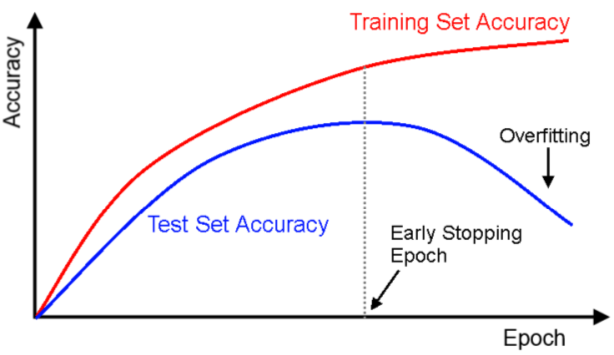
\includegraphics[width=100mm]{Imagenes/early_stopping.png}
    \caption{Representación gráfica deEarly Stopping}
    \label{fig:early_stopping}
    
\end{figure}


